\documentclass[twocolumn]{article}
\usepackage{amsmath}	%paquete matemática
\usepackage{xtab}		%tablas	
\usepackage{graphicx}	%gráficas
\usepackage{subfigure}	%figuras	
\usepackage{fullpage}	%acomodar página
\usepackage{blindtext}	%texto de relleno
\usepackage{hyperref}	%referencias
%\usepackage{multicol}	%columnas

\title{\sc Ecuaciones, tablas y figuras}
\author{Guillermo Arag\'on}
\date{Lunes 04 de Julio}
\pagestyle{empty}


\begin{document}

\thispagestyle{empty}
\maketitle	

\section{Figuras} % (fold)
\label{sec:figuras}

Prueba con im\'agenes de alta calidad aunque no tenga que ver con ciencia, igual sirve para mejorar mi escritura en teclado
	

\blindtext



\vspace{1cm}
En la figura (\ref{fig:Asuka Parche}) \hspace{1cm} se observa a Asuka con un parche.

\begin{figure}[h!]
	\centering
	
\includegraphics[width=0.5\textwidth]{911}
	\caption{Asuka Langley}
	\label{fig:Asuka Parche}
\end{figure}

\begin{figure}[h!]
	\centering
	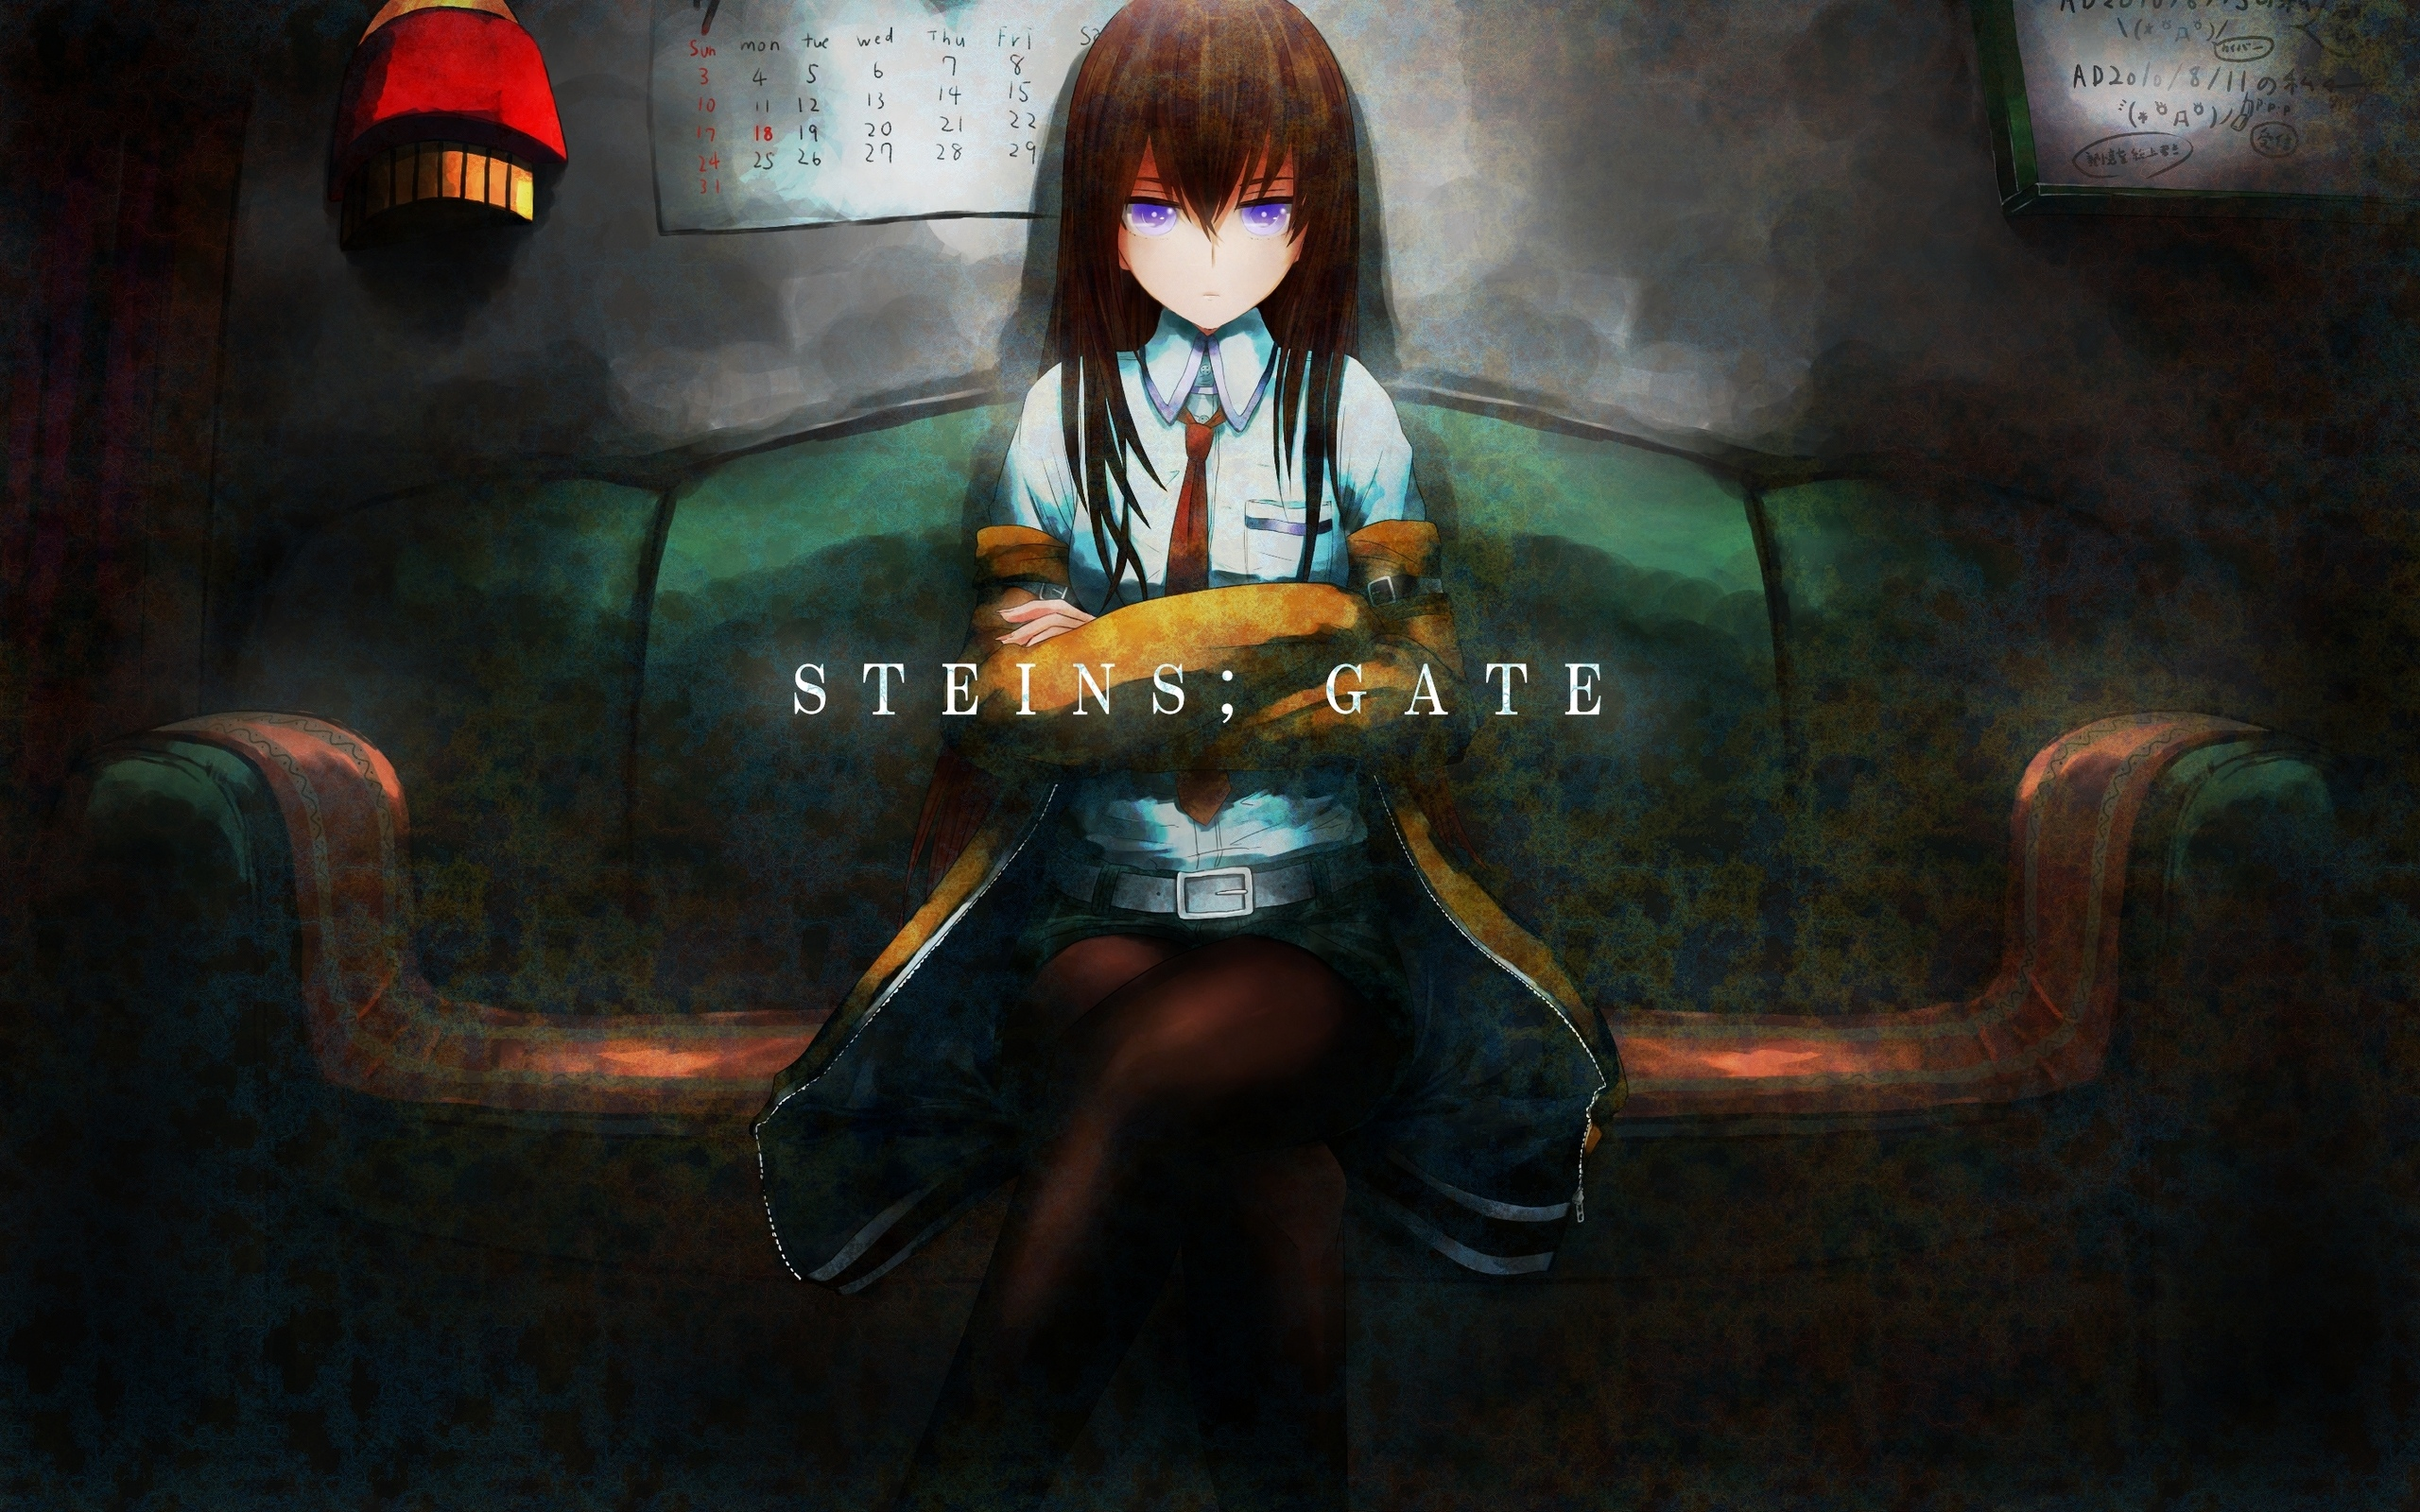
\includegraphics[width=0.5\textwidth]{mk}
	\caption{Mikase Kurisu}
	\label{fig:Mikase Kurisu}
\end{figure}

Para checar como hacer las subfiguras consultar este hipervinculo \href{https://en.wikibooks.org/wiki/LaTeX/Floats,_Figures_and_Captions}{Floats, Figures and Captions}
% section figuras (end)

\section{Equations} % (fold)
\label{sec:equatinons}
Como se obcserv\'o en la secci\'on \ref{sec:figuras} se pueden citar distintos entornos  como figuras o ecuaci\'ones (Eq. \eqref{eq:Area})

\begin{equation}\label{eq:Area}
A=b*h
\end{equation}

% section equatinons (end)

\section{Tabular} % (fold)
\label{sec:tabular}

\begin{center}
	
\begin{tabular}{|||l|c|r|||}
 \hline
 \hline
 \textbf{Nombre} & \textbf{Edad} & \textbf{Estado}\\
 \hline
 \hline
 \hline 
 Reinaldo	&	32	&	Guanajuato\\
 Marcela	&	21	&	Tabasco\\
 Ana 		&	24	&	Tabasco\\
 Guillermo	&	24	&	Quer\'etaro\\
 \hline
 \hline
\end{tabular}

% section tabular (end)
\end{center}
\end{document}